% Section 4.3 should show that for every k, the snowflake tree (with
% vertex weights 1/2+delta and 1/2
% can be realized as a contact graph of disks; and this realization has
% Hausdorff distance at most 1
% from a regular Hexagon (of side length k). Let us also define a
% "canonical position" of the disk
% centers; where each center is a vertex of the hexagonal lattice. Note,
% however, that the canonical
% position does not give a valid realization!
\subsection{Perturbed Weighted Trees $T_\epsilon$}

A perturbed weighted tree $T_\epsilon$ is a weighted unit tree with unit weight on every vertex with the exception of the root vertex having weight $\frac{1}{2}+\epsilon$ where $\epsilon>0$ can be realized as a disk touching graph (a disk arrangement).  

The perturbed snowflake follows the construction of the perfect snowflake with the exception of $v_0$ having weight $\frac{1}{2} + \epsilon$ where $\epsilon > 0$.
A perturbed snowflake realization has some distinct qualities from perfect snowflake realizations.  
The angular relationships between adjacent vertices may vary; the distance between adjacent and neighboring vertices may vary as well.


In general, the perturbation $\epsilon$ can modify the realization of a perfect snowflake $S_i$ in the following ways:
\begin{enumerate}
\item \textbf{Modification of $S_1$.} 

Given a instance of a perturbed snowflake with $v_0$ having weight $\frac{1}{2} + \epsilon$ where $\epsilon > 0$, vertices neighboring $v_0$ each have a range of placement on the plane when realizaed as a disk arrangement. 
Figure \ref{fig:modifiedContactGraph} shows a realization of $S_1$ and illustrates one such example of possible gaps, $\epsilon$, that could be created between adjacent disks of $S_1$ in a perfect snowflake.  

Note that (1) the adjacent disks in a perfect snowflake may or may not be adjacent in a given perturbed snowflake of $S_1$ and (2) $S_1 \subseteq S_i$ for any $i \in \bbN$.  

\begin{lem}\label{lem:s1Small}
For any realized perturbed snowflake $S_i$, the gaps created in subset $S_1 \subset S_i$ are small.
\end{lem}

% Figure \ref{fig:modifiedContactGraph.pdf} shows one realization of a perturbed $S_1$.  
% For any realization of $S_1$, the perturbation $\gamma$ can create gaps, $\epsilon (\gamma)$ between adjacent disks that contact the root disk.  
\item \textbf{Modification of disk placement corresponding to vertices of $p_k$.}
We've shown how the disks can be displaced in $S_1$; for larger snowflakes, the displacement can propogate through the remaining disks of the arrangement.  
The disks can along the paths $p_1$ through $p_6$ may also have displacement as well.  
In canonical position, the disks along paths $p_1$ through $p_6$ will form angles $\alpha_k =\frac{\pi}{3} $ and $\beta_k=\frac{2\pi}{3}$ (see Figure \ref{fig:PerturbedSpine.pdf} for example).  
In noncanonical position, the disks along paths $p_1$ through $p_6$ will form angles that may vary.  

\begin{minipage}{\linewidth}
\begin{center}
\includegraphics[width=.33\columnwidth]{graphics/PerturbedSpine.pdf}
\captionof{figure}{This figure shows a disk arrangement along a path $p_k$ in canoncical position.  Note that perturbation in a snowflake and modify the placement of the disks in such a way that $\alpha_k$ and $\beta_k$ or $\alpha_{k+1}$ and $\beta_{k+1}$ may be of a noncanonical value.}\label{fig:PerturbedSpine.pdf}
\end{center}
\end{minipage}

Our goal here is to show that the change of the angular value of $\alpha_k$ and $\beta_k$ are small:
\begin{lem}\label{lem:angularArrangement}
For any realized perturbed snowflake $S_i$, the angular value of $\alpha_k$ and $\beta_k$ are small.
\end{lem}

\item \textbf{Modification of disk placement along corresponding to the $p_{k,j}^\text{th}$ vertex of $S_i$.}  
For the $\jth$ disk along the $\kth$ path $p_{k,j}^+$ or $p_{k,j}^-$, perturbation can displace the postion of the disk on the plane and the angular relationship of the neighboring disks (see Figure \ref{fig:PerturbedVertebrae.pdf} for example). 

\begin{minipage}{\linewidth}
\begin{center}
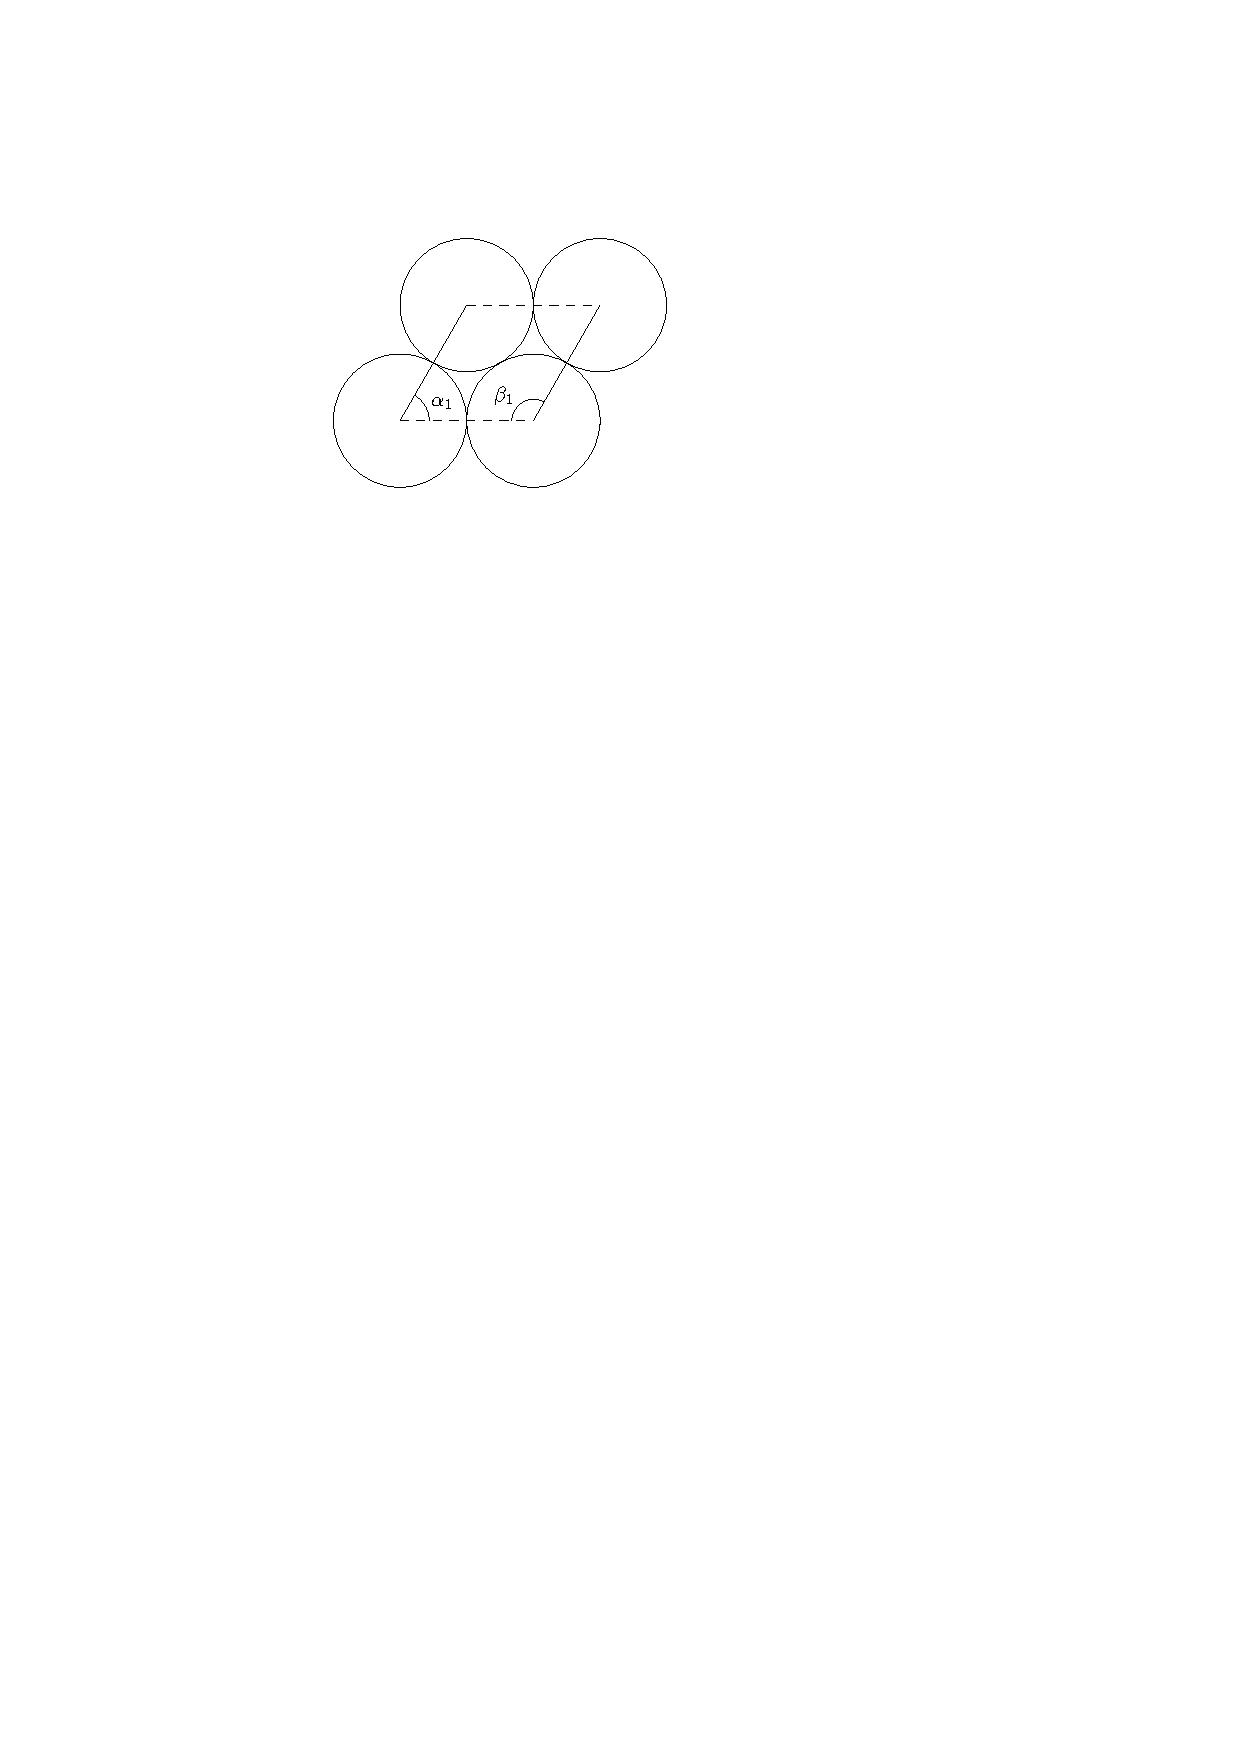
\includegraphics[width=.33\columnwidth]{graphics/PerturbedVertebrae.pdf}
\captionof{figure}{This illustration the relationship angular relationships between neighboring disks $D_{k,j}$, $D_{k+1,j}$, $D_{k+1,j+1}$, and $D_{k,j+1}$.}\label{fig:PerturbedVertebrae.pdf}
\end{center}
\end{minipage}

In this case we will show that the distances between the centers of neighboring disks are small relatively to canonical position of a perfect snowflake, i.e.
\begin{lem}\label{lem:disksOfPathways}
For any realized perturbed snowflake $S_i$, the distance between disks $D_{k,j}$, $D_{k+1,j}$, $D_{k+1,j+1}$, and $D_{k,j+1}$ are relatively small with respect to the relative distance in a perfect snowflake where $k = 1$, $\dots$, $6$ and $j = 2$, $\dots$, $i$.
\end{lem}
\end{enumerate} 

We will show the proofs of Lemmas \ref{lem:s1Small} through \ref{lem:disksOfPathways} later on.


% In Figure \ref{fig:modifiedContactGraph.pdf}, we have a realization of disk arrangement from a perturbed snowflake.
% In a disk arrangement of a perfect snowflake, the disks around the central disk contact the adjacent disks.
% The disk arrangement from the perturbed snowflake does not have this quality.  
% Figure \ref{fig:modifiedContactGraph.pdf} shows a gap $\epsilon(\gamma)$ between adjacent disks around the central disk.  
% This gap is formed from the perturbed weight $\frac{1}{2} + \gamma$ of the central disk.  
% \begin{equation}\label{eqn:epsilonGamma}
% \epsilon(\gamma)=2\gamma + \gamma^2
% \end{equation}
% As the perturbed snowflake grows outer layers, we can begin to define parts of the snowflake and the corresponding disk arrangement.  
% Let the arms extending from the center of a snowflake be \textit{dendrites} and the arms extending off of arms be \textit{metadendrites}.
% In a perturbed snowflake, the dendrites and metadendrites have some freedom to about the plane.  our
% \begin{minipage}{\linewidth}
% \begin{center}
% \includegraphics[width=.66\columnwidth]{graphics/PerturbedContactGraphAnatomy.pdf}
% \captionof{figure}{}\label{fig:PerturbedContactGraphAnatomy.pdf}
% \end{center}
% \end{minipage}
% In Figure \ref{fig:PerturbedContactGraphAnatomy.pdf}, we show an overlay of a realization of a perturbed snowflake, a corresponding disk arrangement, and concentric hexagons about the $v_0$.




% \begin{lem}\label{lem:cg-1}
% Given any realization of a perturbed snowflake of 7 weighted vertices, with the central vertex $v_0$ weighted $\frac{1}{2} + \gamma$ and the others weighted $\frac{1}{2}$, the total additional distance between all vertices is $6 \epsilon(\gamma)$ compared to a perfect snowflake of 7 unit weight vertices.
% \end{lem}
% \begin{proof}
% Consider a canonical disk arrangement of a perturbed snowflake of 7 weighted vertices (see Figure \ref{fig:modifiedContactGraph.pdf}).
% The side length of the sides formed between the center of the central disk and two adjacent disks around the central disk is $1 + \gamma$.  
% Let the distance between the two adjacent disks be $1 + \epsilon(\gamma)$.
% There are a total of $6 \epsilon(\gamma)$ between adjacent centers of disks. 
% The total perimeter of the hexagon formed about the centers of the disks in contact with the central disk is $6 + 6\epsilon(\gamma)$. 
% Note that 1) the total perimeter of the hexagon formed on a perfect snowflake of 7 weighted vertices is 6 and 2) the canonical disk arrangement can be transformed to any other disk arrangement corresponding to the perturbed snowflake of 7 weighted vertices by pushing the the ring of disks around the central disk together such that all adjacent disks are in contact with each other with the exception of the disks at the end.
% \end{proof}

%  \section{On the Decidability of Problem \ref{problem:UnorderedContactGraph}}
% \begin{proof} 
% Consider a $k \times (\sqrt{3}k)$ rectangle section of a triangular lattice, and place disks of radius 1 at each grid point as in Fig. ?????. 
% The contact graph of these disks contains 2-cycles. 
% Consider the spanning tree $T$ of the contact graph indicated in Fig. ????. 
% The tree $T$ decomposes into paths of collinear edges: $T$ contains two paths along the two main diagonals, each containing $2k - 1$ vertices; all other paths have an endpoint on a main diagonal. 
%  We now modify the disk arrangement to ensure that its contact graph is $T$. 
%  The disks along the main diagonal do not change. 
%  We reduce the radii of all other disks by a factor of $1 - k^{-3}$ (as a result, they lose contact with other disks), and then successively translate them parallel in the direction of the shortest path in $T$ to the main diagonal until the contact with the adjacent disk is reestablished. 
%  The Hausdorff distance between the union of these disks and the initial $k \times (\sqrt{3}k)$ rectangle is clearly less than 1.
%  However, the contact tree $T$ with these radii no longer has a unique realization (small perturbations are possible). 
%  To show stability, we argue by induction on the hop distance from the central disk. 
%  There are $O(i)$ disks at i hops from the central disk, most one which have radius $(1-k^{-3}) \frac{1}{2}$.
%  Since all radii are 1 or $(1-k^{-3}) \frac{1}{2}$,the six neighbors of the central disk can differ from the regular hexagon by at most $O(k )$. 
%  Similarly, the disks at $i$ hops from the center be off from the triangular grid pattern by $O(i2^{k-3})$, for $i = 1,2,\dots,k$.

%  \begin{minipage}{\linewidth}
% \begin{center}
% \includegraphics[width=.66\columnwidth]{graphics/ch4Paralellogram.pdf}
% \captionof{figure}{}\label{fig:ch4Paralellogram.pdf}
% \end{center}
% \end{minipage}
% \end{proof}


% Recall that problem (\ref{problem:UnorderedTree}) states: given a positive weighted tree, $T$, is $T$ the contact graph of some disk arrangement where the radii are equal to the vertex weights?  

% \begin{proof}
% Suppose we are given a positive weighted tree, $T = \lr{V_1,E_1}$.  By the Disk Packing Theorem, there is a disk arrangement in the plane, $D$, whose contact graph, $G=\lr{V_2,E_2}$ is isomorphic to $T$.  We need to so that $G=T$ and the radii of the disks in $D$ are equal to the vertex weights of $T$.

% To show that $G=T$, we need to show that $V_1=V_2$ and $E_1=E_2$.  

% To show that the radii of the disks in $D$ are equal to the vertex weights of $T$, we first consider ....  
% \end{proof}

% Related Previous Work. Polygonal linkages (or body-and-joint frameworks) are a gen-
% eralization of classical linkages (bar-and-joint frameworks) in rigidity theory. A linkage
% is a graph G = (V, E) with given edge lengths. A realization of a linkage is a (crossing-
% free) straight-line embedding of G in the plane. Bhatt and Cosmadakis [3] proved that
% the realizability of linkages is NP-hard. Their “logic engine” method [11, 13, 15, 18],
% has become a powerful tool in graph drawing. The logic engine is a graph composed
% of rigid 2-connected components, connected by cut vertices (hinges). The two possi-
% ble realizations of each 2-connected component (that differ by a single reflection) rep-
% resent the truth assignment of a binary variable. This method does not applicable to
% the oriented version of the realizability, where the circular order of the neighbors of
% each vertex is part of the input. Cabello et al. [6, 14] proved that the realizability of 3-
% connected linkages (where the orientation is unique by Steinitz’s theorem) is NP-hard,
% but efficiently decidable for near-triangulations [6, 12].
% Note that every tree linkage can be realized in R2 (with almost collinear edges).
% According to the celebrated Carpenter’s Rule Theorem [9, 21], every realization of a
% path (or a cycle) linkage can be continuously moved (without self-intersection) to any
% other realization. In other words, the realization space of such a linkage is always con-
% nected. However, there are trees of maximum degree 3 with at few as 8 edges whose
% realization space is disconnected [2]; and deciding whether the realization space of a
% tree linkage is connected is PSPACE-complete [1]. (Earlier, Reif [20] showed that it is
% PSPACE-complete to decide whether a polygonal linkage can be moved from one re-
% alization to another among polygonal obstacles in R3.) Cheong et al. [7] considers the
% “inverse” problems of introducing the minimum number of point obstacles to reduce
% the configuration space of a polygonal linkage to a unique realization.
% Connelly et al. [10] showed that the Carpenter’s Rule Theorem generalizes to certain
% polygonal linkages, which are obtained by replacing the edges of a path linkage with
% special polygons called (slender adornments). Our Theorem 1 indicates that if we are
% allowed to replace the edges of a path linkage with arbitrary convex polygons, then
% deciding whether the realization space is empty or not is already NP-hard.
% Recognition problems for intersection graphs of various geometric object have a
% rich history [18]. Breu and Kirkpatrick [5] proved that it is NP-hard to decide whether
% a graph G is the contact graph of unit disks in the plane (a.k.a. recognizing coin graphs
% is NP-hard). A simpler proof was later provided via the logic engine [13]. It is also NP-
% hard to recognize the contact graphs of pseudo-disks [18] and disks of bounded radii [4]
% in the plane, and unit disks in higher dimensions [17, 18]. All these hardness reductions
% produce graphs of high genus, and do not apply to trees. Note that the contact graphs
%  of disks (of arbitrary radii) are exactly the planar graph (by Koebe’s circle packing
%  theorem), and planarity testing is polynomial. Consequently, every tree is the contact
%  graph of disks of some radii in the plane.


%My goals for next week are as follows:
%1) Clean up chapter 1.  This will happen over the next several weeks.
%2) Continue section 2.3
%3) Add graphics to epsilon-approximation definition to facilitate the explanation.
%4) Anything else  I have time for.



% $\overline{v_0 }$

%Define the snowflake graph, S_i, without pictures
%v_0 has six paths attached to it, p_1, p_2, ..., p_6.  Each path has i vertices.
%for every other path p_1, p_3, and p_5 ,
%	Each vertex on that path has two paths attached, one path on each side of p_k.
%	The number of vertices that lie on the path attached to the j^{th} vertex of p_k is $i-j$
%Let all vertices on the contact graph have weight 1 except $v_0$ whose weight is 1 + \epsilon.
%For any $i$, the weighted contact graph $S_i$, is a subgraph of the unit distance graph of the triangular lattice
%lattice be V = {a(1,0) + b(1/2, \frac{\sqrt{2}}{3} such that a,b \in \bbZ}
%		  E = {{u,v} such that u,v \in V and ||u-v||=1}
%Define this as a canonical position of the disks corresponding to the vertices; goal: show every realization of S_i's disks is close to the canonical position of the disk under hausdorff distance (see lemma)
%NTS: there exists a disk arrangement that corresponds to this weighted contact graph, S_i
%pf:For any two adjacent stems are disjoint, angular displacement and planar (point) displacement
  

%    \begin{prob}[Unordered Realizibility Problem for the Tree]\label{problem:UnorderedTree}
%    For a tree with positive weights for the verticies, it asks whether it is a contact graph of some 
%    disk arrangement where the radii are equal to the vertex weights.
%    \end{prob}
%    
%    \begin{prob}[Ordered Realizibility Problem for the Tree]\label{problem:OrderedTree}
%    For a tree with positive weights for the vertices, it asks whether its corresponding graph is the 
%    ordered contact graph of some disk arrangement where the radii equal the vertex weights.
%    \end{prob}